
%{\tt asdf}

\section{Running Sampler}

\subsection{About Sampler}
 \begin{itemize}
  \item If you are happy with the results of the Bertini\_real decomposition, you may wish to refine the triangulation of the surface or curve. This can be acheived using the \texttt{sampler} program after calling \texttt{bertini\_real}. Sampler can be used on both curves and surfaces. 
  \item This section will show you how to:
   \begin{enumerate}
   	\item Properly run sampler, with visual examples
   	\item Use the different algorithms to shape curves and surfaces
   	\item Use matlab to better visualize curves and surfaces
   \end{enumerate}
 \end{itemize}  

 \subsection{Curves}
 \label{sec:sampler_curve}

 	\subsubsection{Running Sampler (Using an Example)}
 	 In order to show how to properly run sampler, I will be using an example of a curve, going through each step to make sure the basics of sampler are covered.
 \begin{longtabu} to \textwidth {
 X[1,c,m]
 X[1,c,m]}
\hline
\rowfont\bfseries
\textbf{Instructions} & \textbf{Screen Shot} \\
\hline  \\ 
\endfirsthead
\caption[]{\textit{Continued from previous page}}\\
\hline
\textbf{Instructions} & \textbf{Screen Shot} \\
\hline \\
\endhead
\bottomrule \multicolumn{2}{r}{\textit{Continued on next page}} \\
\endfoot
\bottomrule \multicolumn{2}{r}{\textit{}} \\
\endlastfoot
First, choose the curve you wish to produce. (In this case I am choosing the {\tt eistute\_sphere}, which is found in the {\tt intersections} file which can be found in the {\tt zoo} file) & 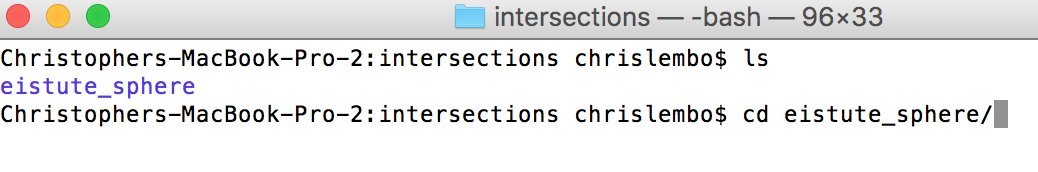
\includegraphics[width=0.4\textwidth]{curvesampler1}  \\  \\  \\
\hline \\
Invoke {\tt bertini} and {\tt bertini\_real} by entering in each on the command line individually & 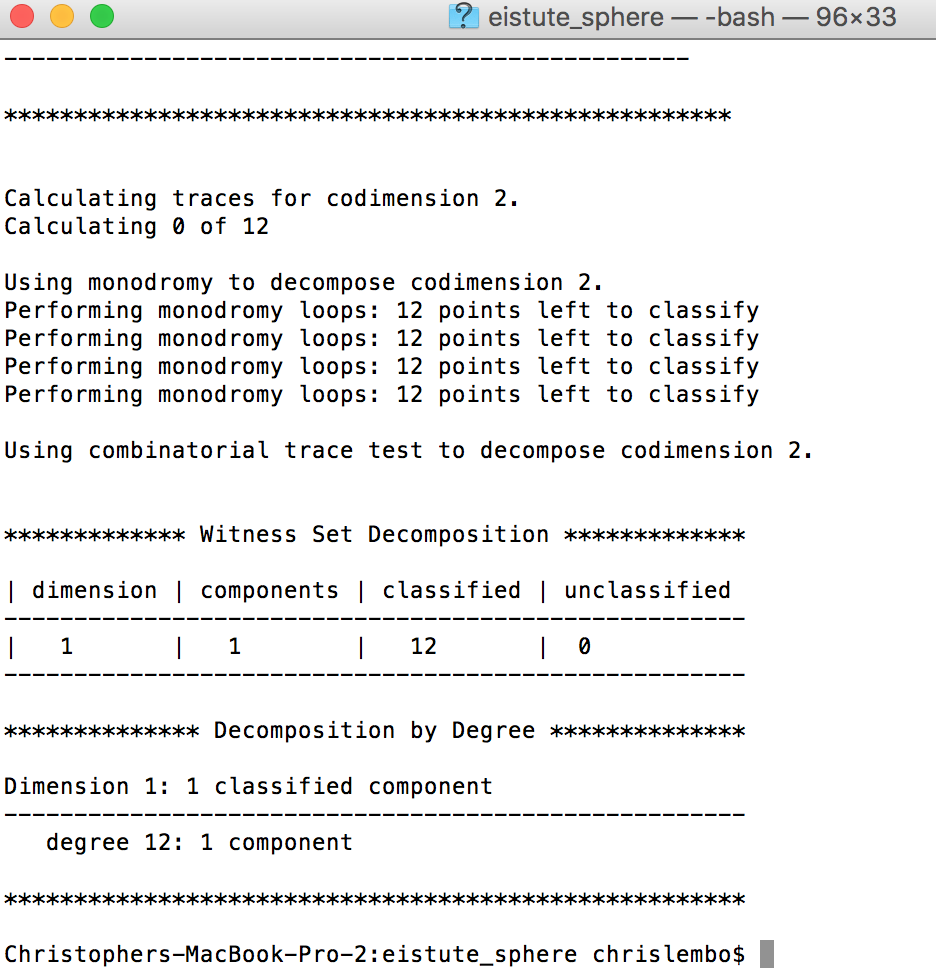
\includegraphics [width=0.4\textwidth]{curvesampler2} \\ \\ \\ 
\hline \\
Invoke {\tt sampler} by entering it in on the command line & 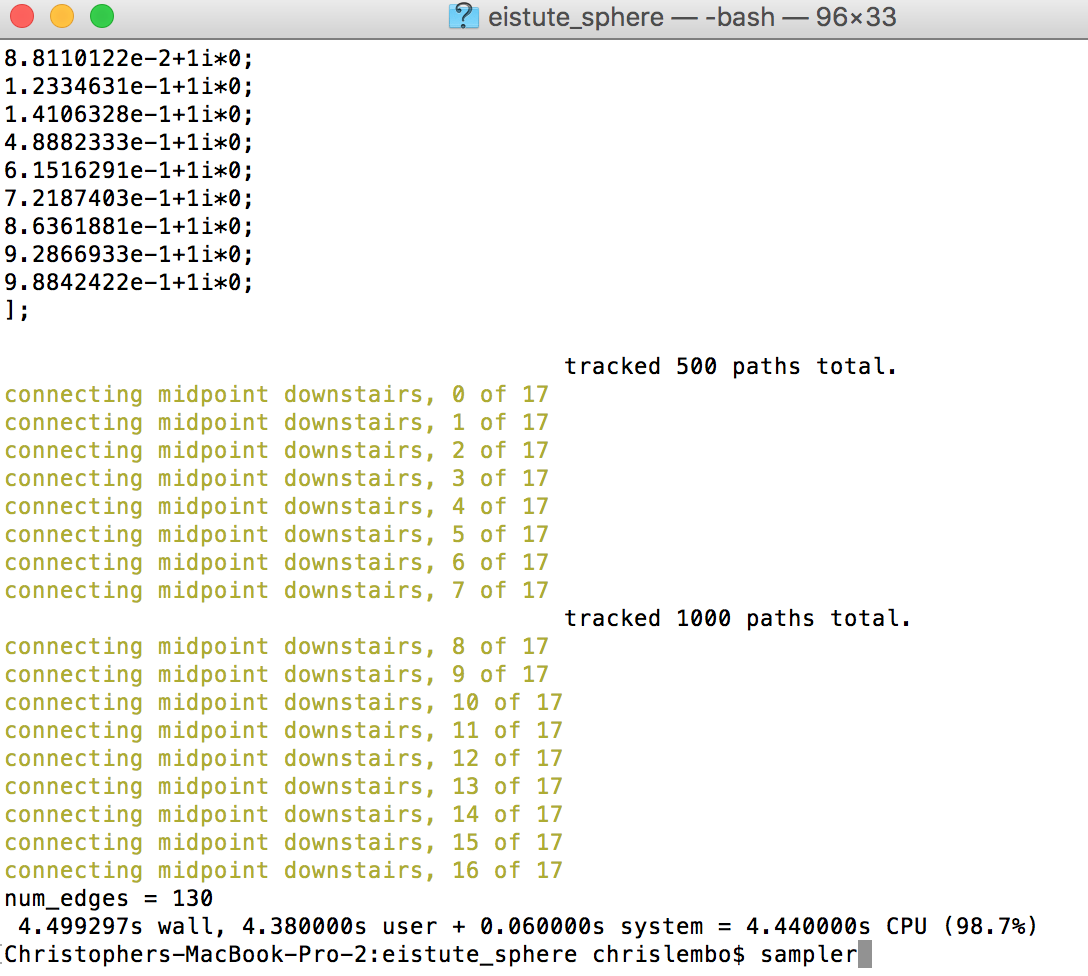
\includegraphics [width=0.4\textwidth]{curvesampler3} \\ \\ \\
\hline \\ 
Now use Matlab to produce the image of the curve
\begin{enumerate} 
	\item Go to the folder that holds your curve, then type {\tt gather\_br\_samples}
	\item To produce the image, type in {\tt bertini\_real\_plotter}
	\item you should end up with a figure along with matlab's display of viewing options
\end{enumerate}
& 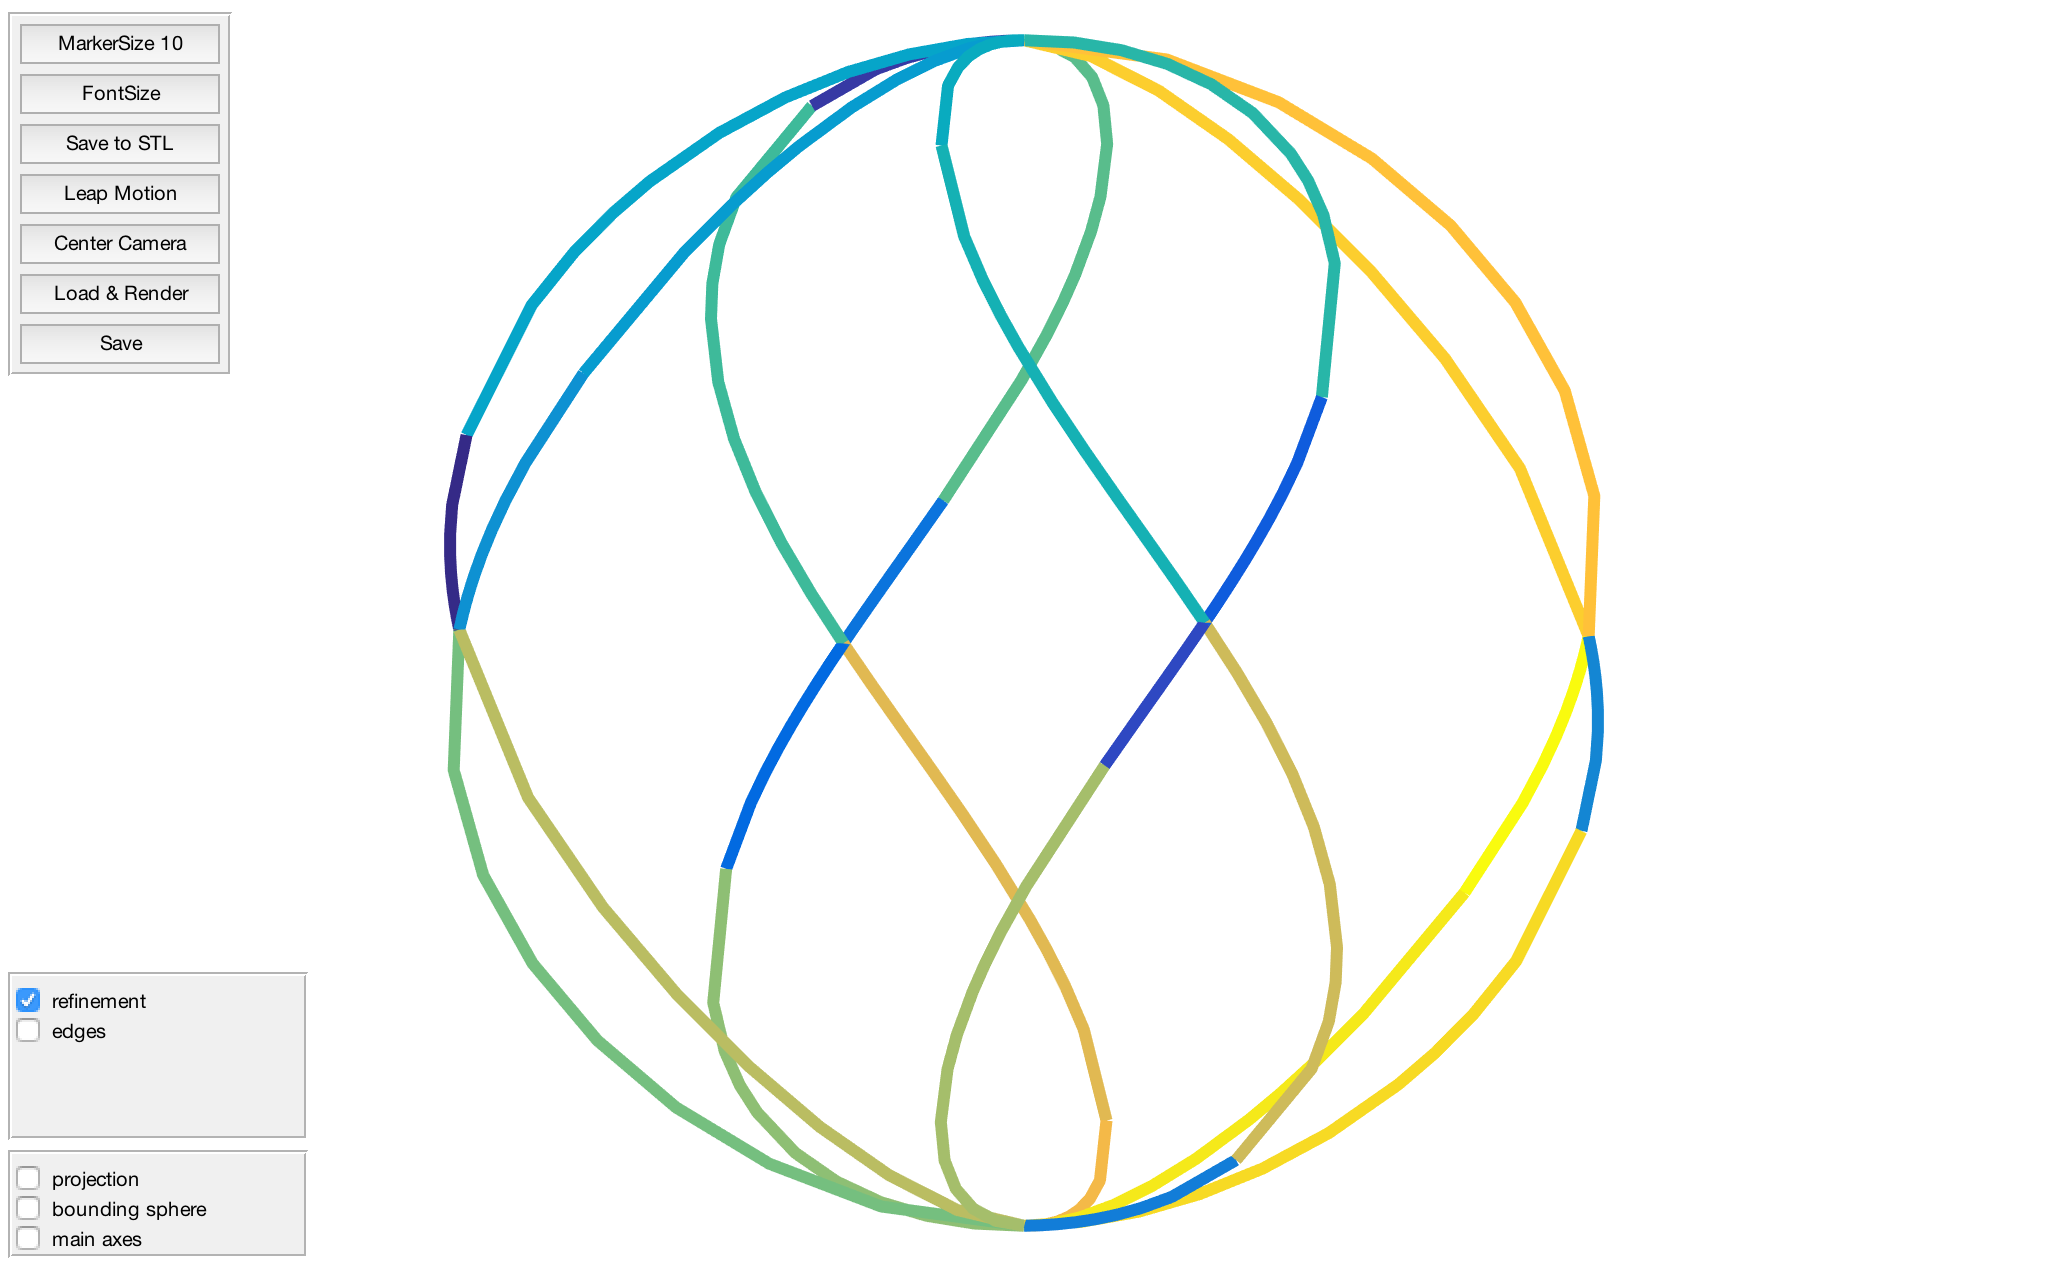
\includegraphics [width=0.4\textwidth]{curvesampler4.png} \\ \\ \\ 
  
\end{longtabu}


 	\subsubsection{Available curve sampling algorithms}
 	

 	There are three curve sampling algorithms available in the Sampler module for Bertini\_real.

 	\begin{enumerate}

 		\item {\tt -m a} -- Adaptive -- by movement of a predicted point.  Default choice.

 		\item {\tt -m d} -- Adaptive -- by distance between consective samples

 		\item {\tt -m f} -- Fixed -- every edge gets the same number of points

 	\end{enumerate}

The modes are accessed by calling sampler with the appropriate mode switch.


\paragraph{Curve sampling algorithm: Adaptive by movement}

This algorithm refines edge-by-edge until the predicted point, and the computed point, are close to each other.  It reduces sample density in regions of the curve which are flat, and has higher density in regions of high curvature.


\begin{figure}[H]
\begin{center}
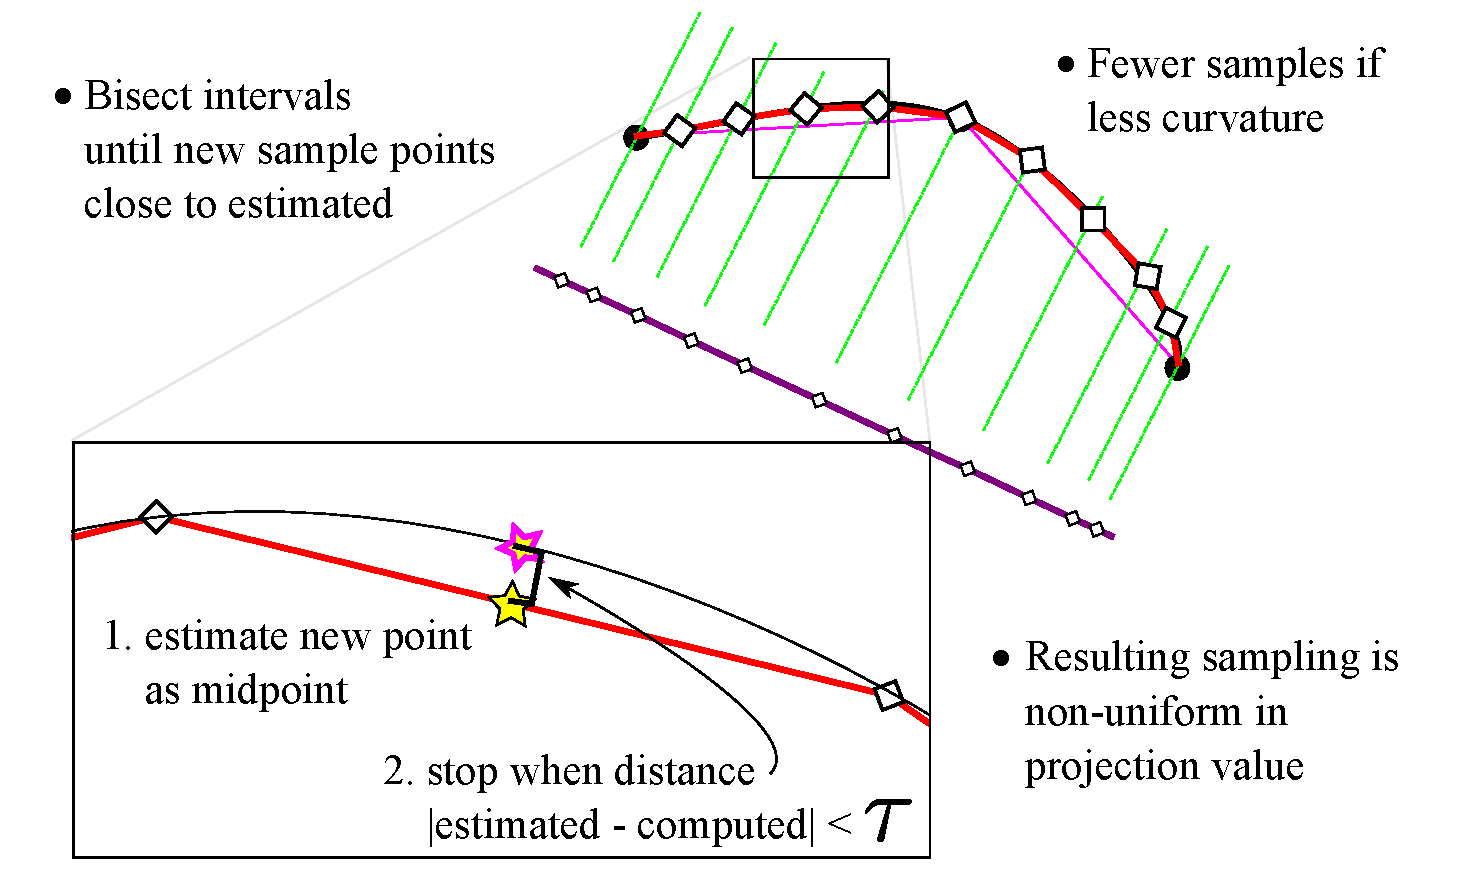
\includegraphics[scale = 0.4]{curve_sampling_adaptive_movement}
\caption[Adaptive-movement curve sampling]{Sampling a curve using movement-adaptive method.  New points are computed on the curve by bisecting intervals until the distance between the estimated midpoint and actual midpoint is less than convergence threshold $\tau$.}
\end{center}
\end{figure}
 
\begin{figure}[H]
\centering
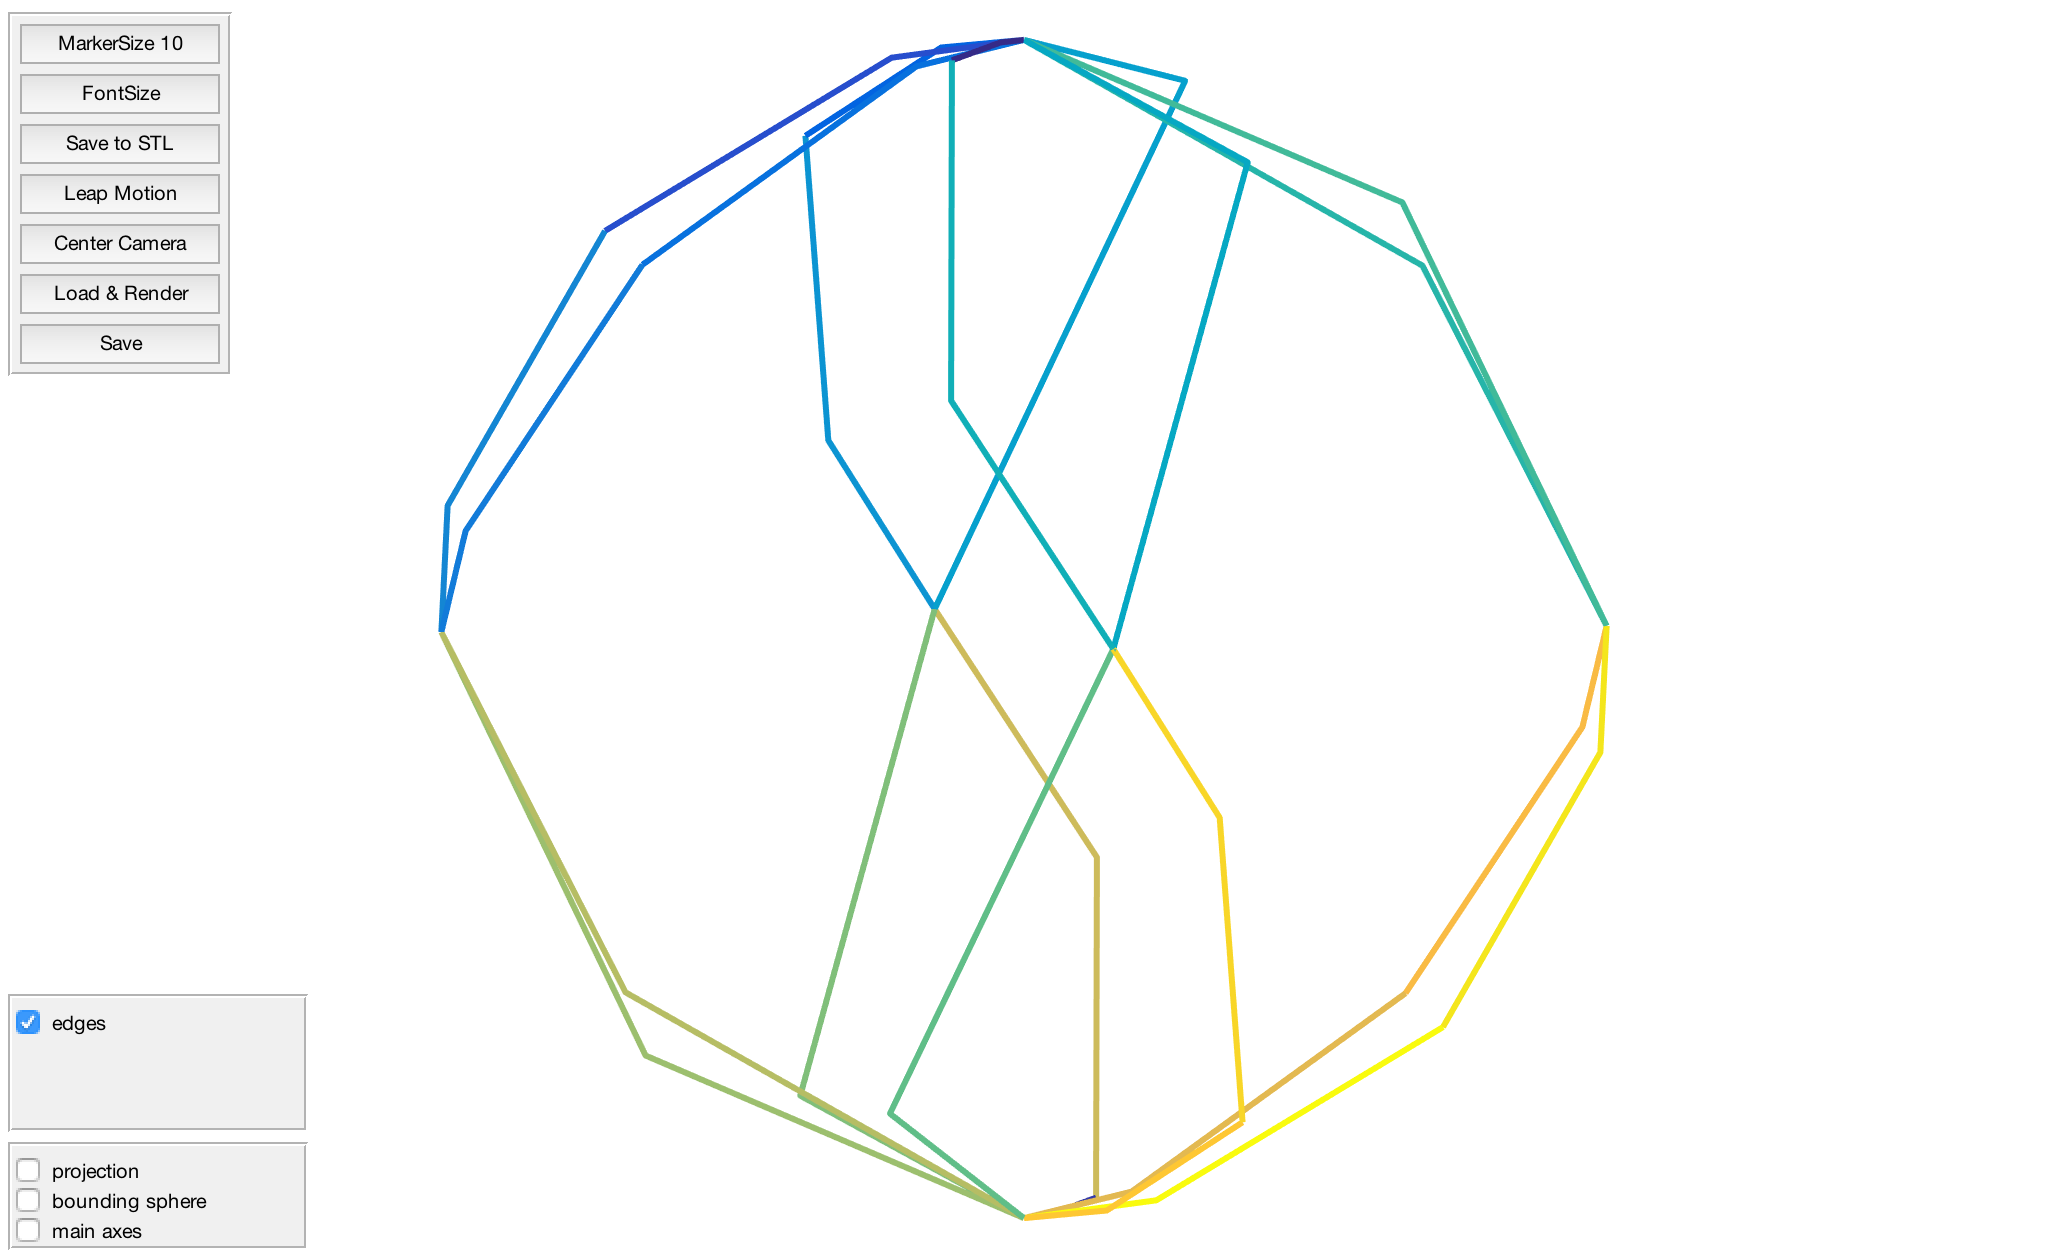
\includegraphics[width=0.5\textwidth]{curvesampler_adm.png}
\caption{This is an example of sampling a curve using the adaptive by movement mode. To replicate this, when invoking sampler, type in {\tt sampler -m a}}
\end{figure}

\paragraph{Curve sampling algorithm: Adaptive by distance}

The adaptive-by-distance refinement algorithm refines the edge by bisection until the distance between consecutive samples is less than some user-set threshold, or a maximum number of refinement iterations has been computed.  This algorithm works well, but over-samples flat regions of the curve, where relatively few points should be necessary.  


\begin{figure}[H]
\begin{center}
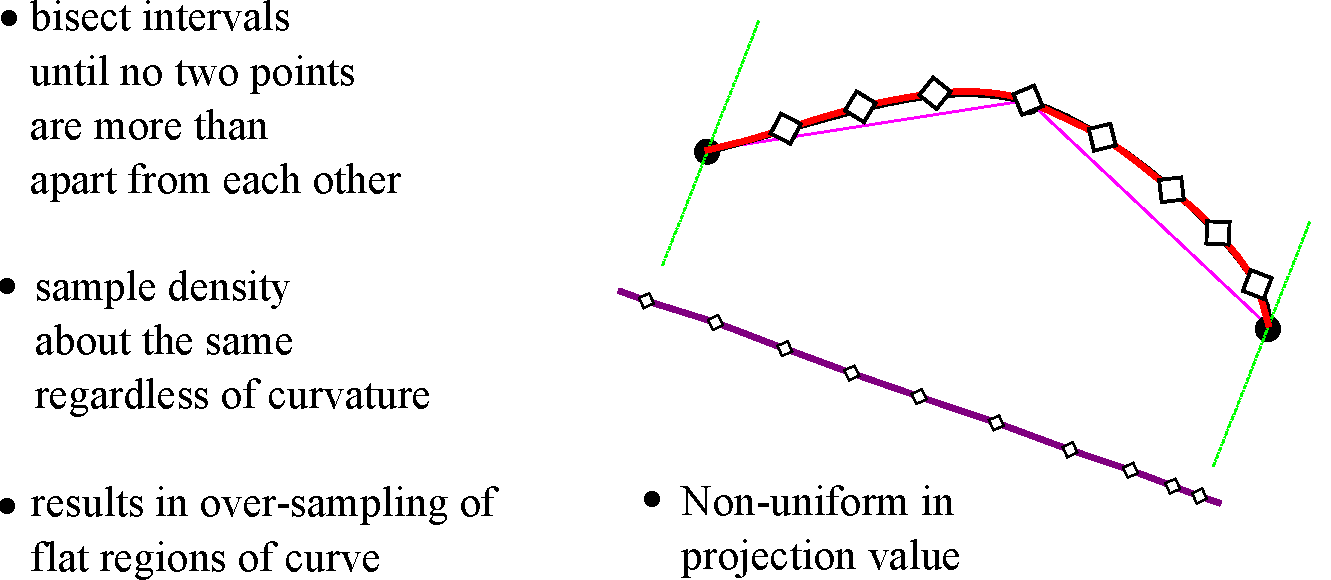
\includegraphics[scale = 0.4]{curve_sampling_adaptive_distance}
\caption[Adaptive-distance curve sampling]{Sampling a curve using distance-adaptive method.  New points are computed on the curve by bisecting intervals for which the distance between consecutive samples is larger than the convergence threshold $\tau$.}
\end{center}
\end{figure}

\begin{figure}[H]
\centering
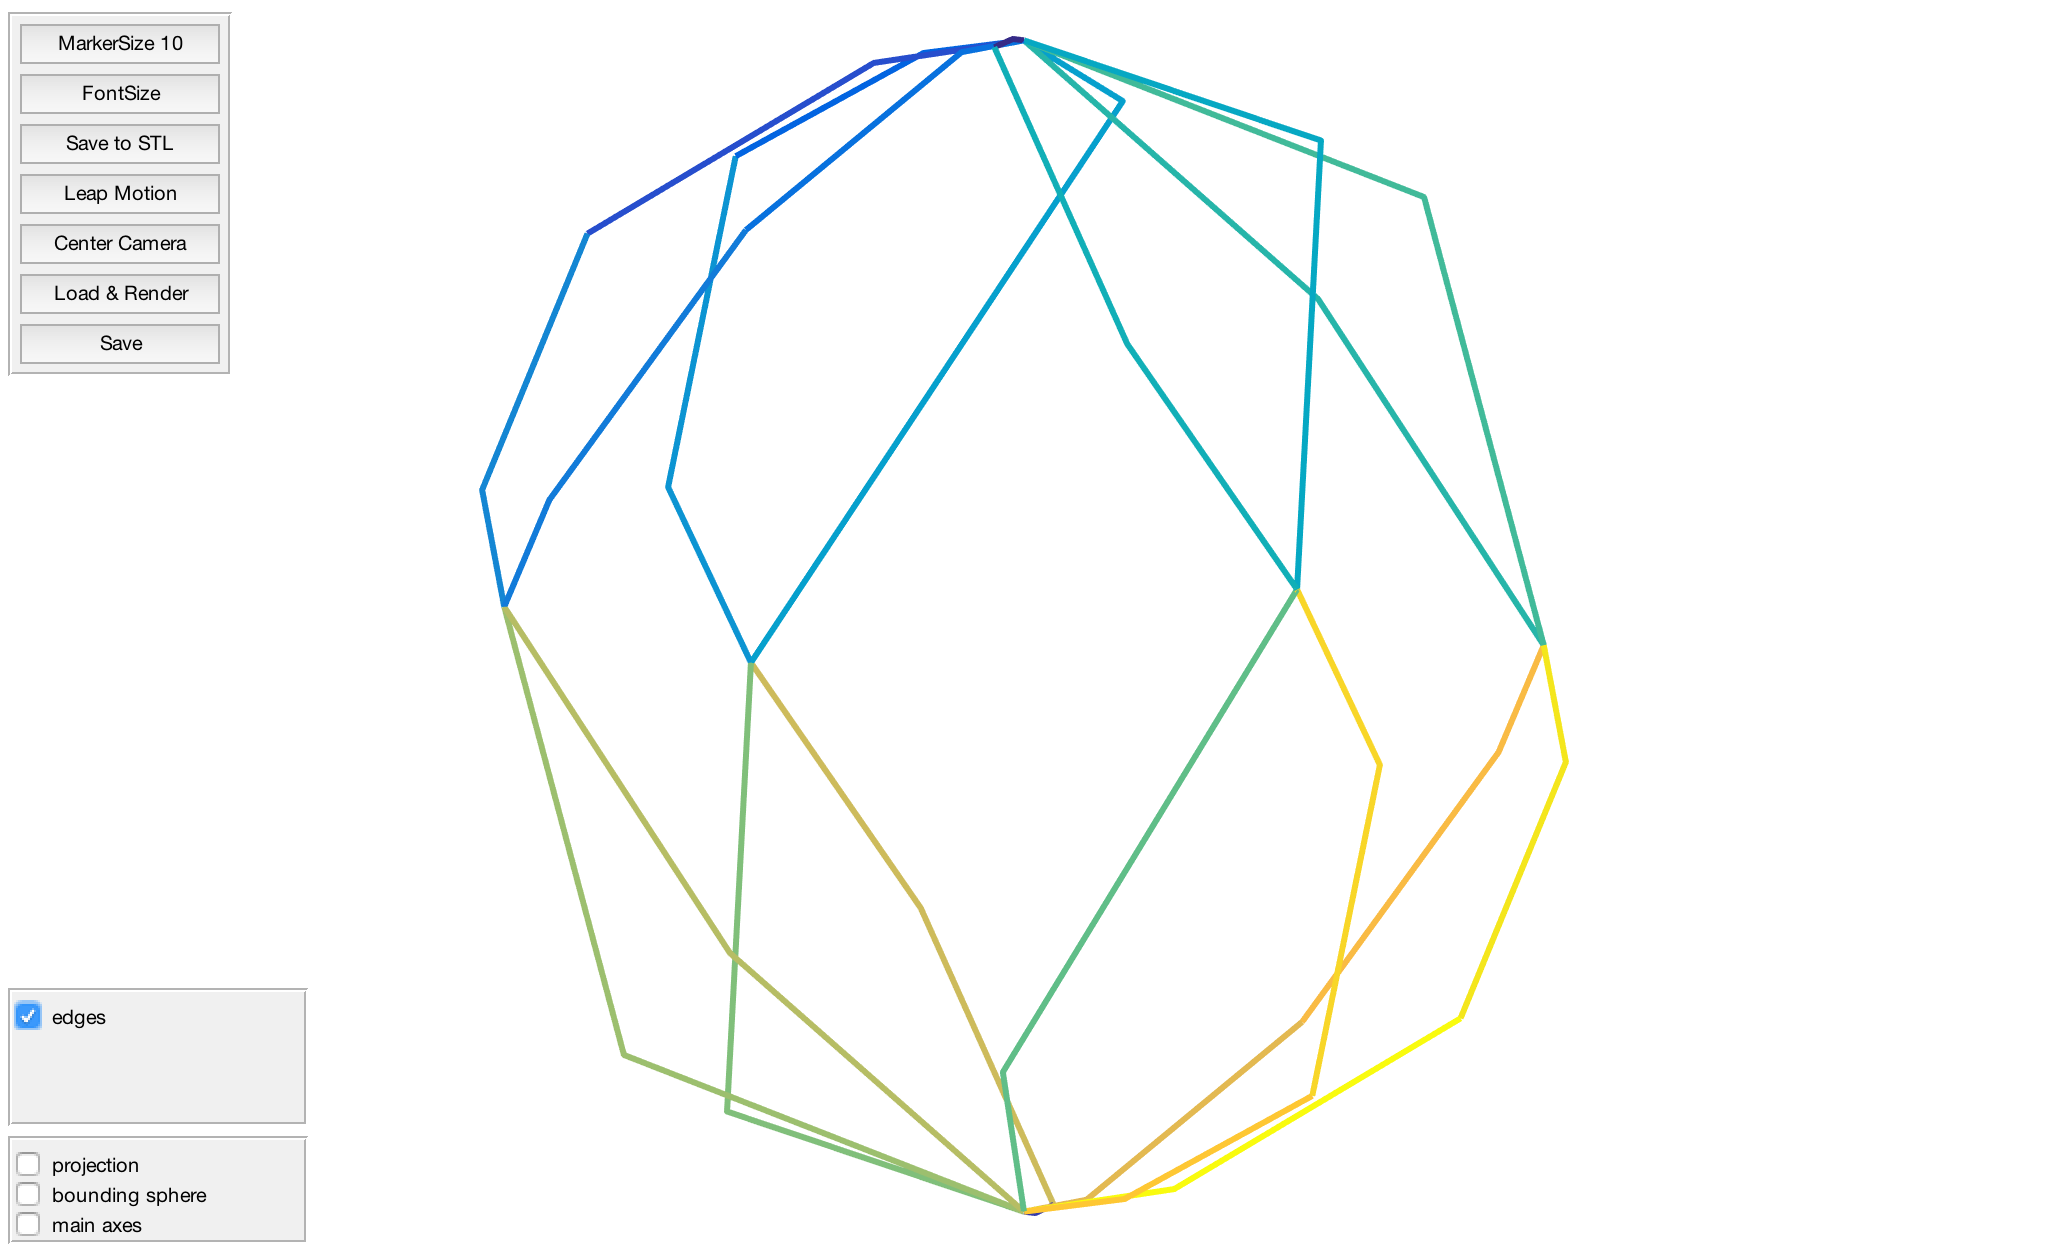
\includegraphics[width=0.5\textwidth]{curvesampler_add.png}
\caption{This is an example of sampling a curve using the adaptive by distance mode. To replicate this, when invoking sampler, type in { \tt sampler -m d}}
\end{figure}



\paragraph{Curve sampling algorithm: Fixed number}

This curve sampling algorithm produces a fixed (by the user) number of sample points per edge of the decomposed curve.  


\begin{figure}[H]
\begin{center}
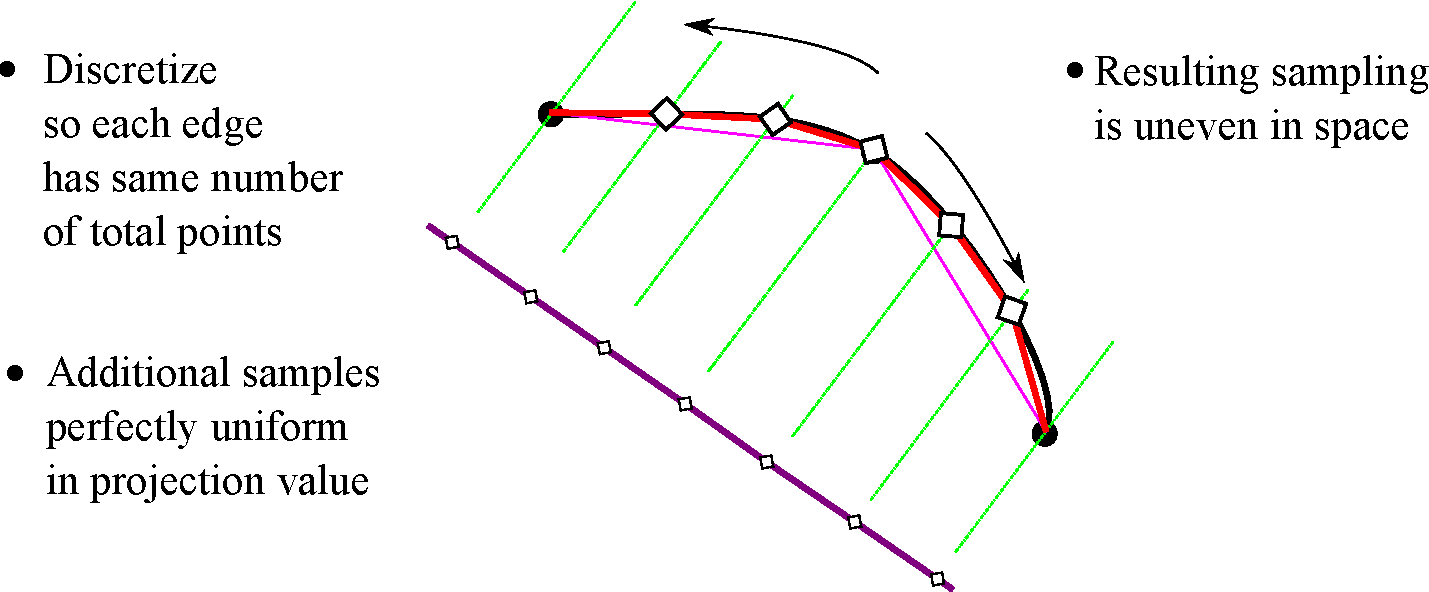
\includegraphics[scale = 0.4]{curve_sampling_fixed}
\caption[Fixed-number sampling of a curve -- how it works]{Fixed-number sampling of a curve.  The midpoint is homotoped so that a fixed number of sample points are computed on each edge of the curve.  The sample points are spaced uniformly in projection value, not in space.}
\end{center}
\end{figure}

\begin{figure}[H]
\centering
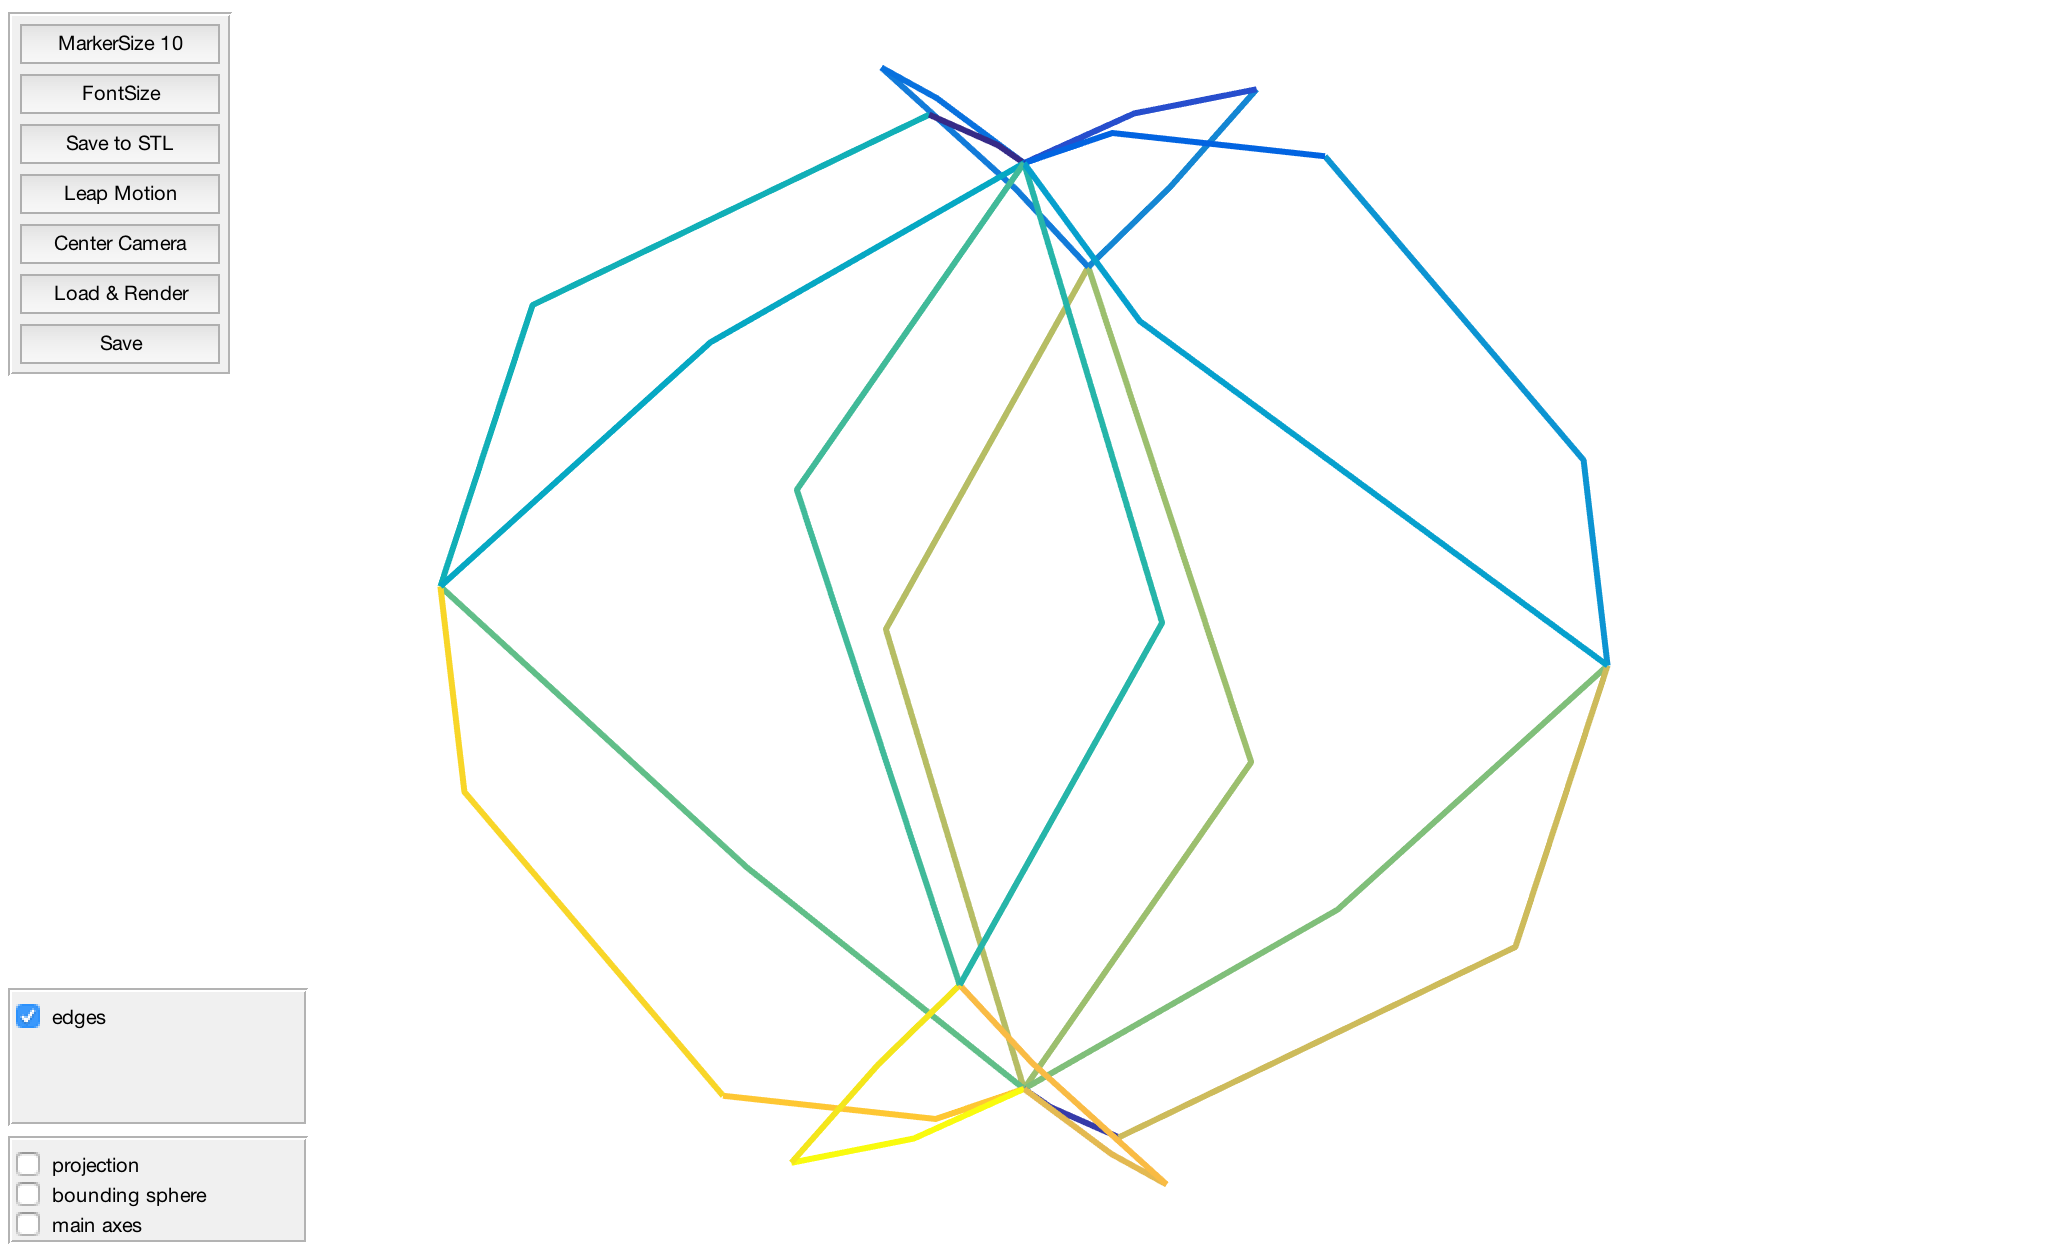
\includegraphics[width=0.5\textwidth]{curvesampler_f.png}
\caption{This is an example of sampling a curve using fixed mode. To replicate this, when invoking sampler, type in {\tt sampler -m f}}
\end{figure}

\subsection{Surfaces}
\label{sec:sampler_surface}

\subsubsection{Running Sampler (Using an Example)}

This section will guide you through running sampler using a surface. One thing to note is that it may take longer to invoke the sampler when using it on surfaces due to the amount of computation being done.

\begin{longtabu} to \textwidth {
 X[1,c,m]
 X[1,c,m]}
\hline
\rowfont\bfseries
\textbf{Instructions} & \textbf{Screen Shot} \\
\hline  \\ 
\endfirsthead
\caption[]{\textit{Continued from previous page}}\\
\hline
\textbf{Instructions} & \textbf{Screen Shot} \\
\hline \\
\endhead
\bottomrule \multicolumn{2}{r}{\textit{Continued on next page}} \\
\endfoot
\bottomrule \multicolumn{2}{r}{\textit{}} \\
\endlastfoot
First, choose the surface you wish to produce. (In this case I am choosing the {\tt sphere}, which is just found in the surfaces file. Once you enter into this file, you are ready to invoke:
\begin{itemize} 
\item {\tt bertini} 
\item {\tt bertini\_real} 
\item {\tt sampler}
\end{itemize} & 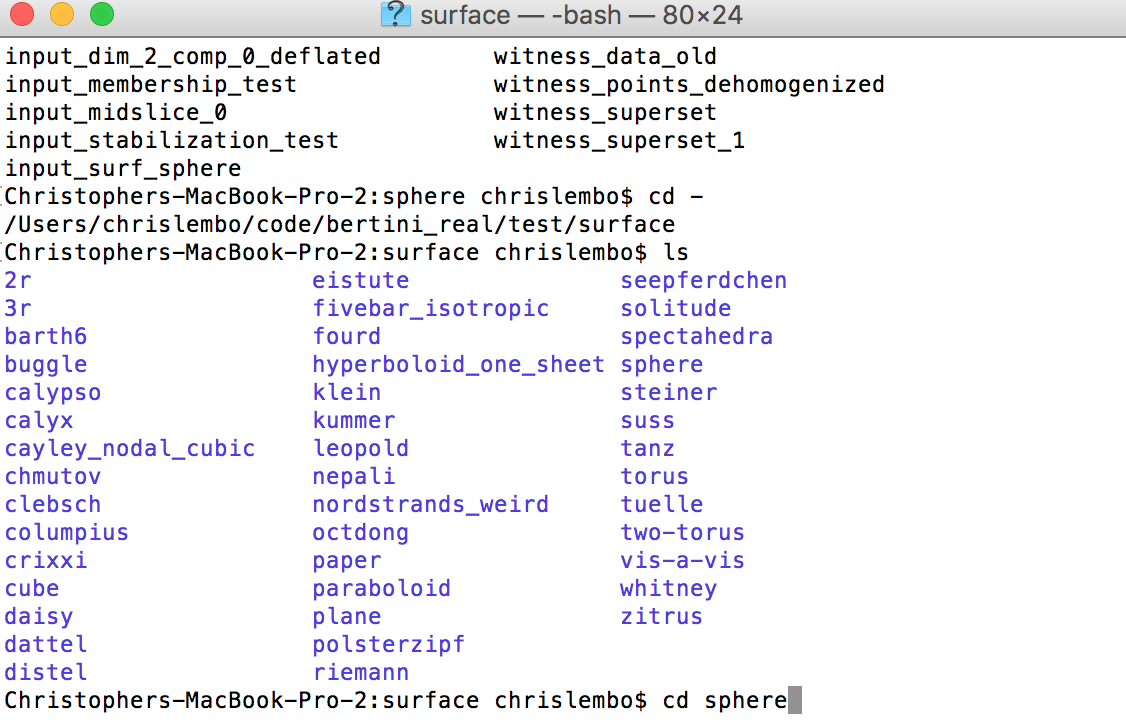
\includegraphics[width=0.4\textwidth]{surfacesampler1}  \\  \\  \\
\hline \\
Once sampler has been invoked, go to matlab and follow the same steps layed out for the sampler curve process, by gathering and plotting. Depending on refinements, you will end up with a sphere with fewer or more points. Here are the two matlab commands:
\begin{itemize} 
\item {\tt gather\_br\_samples} 
\item {\tt bertini\_real\_plotter}
\end{itemize}
 & 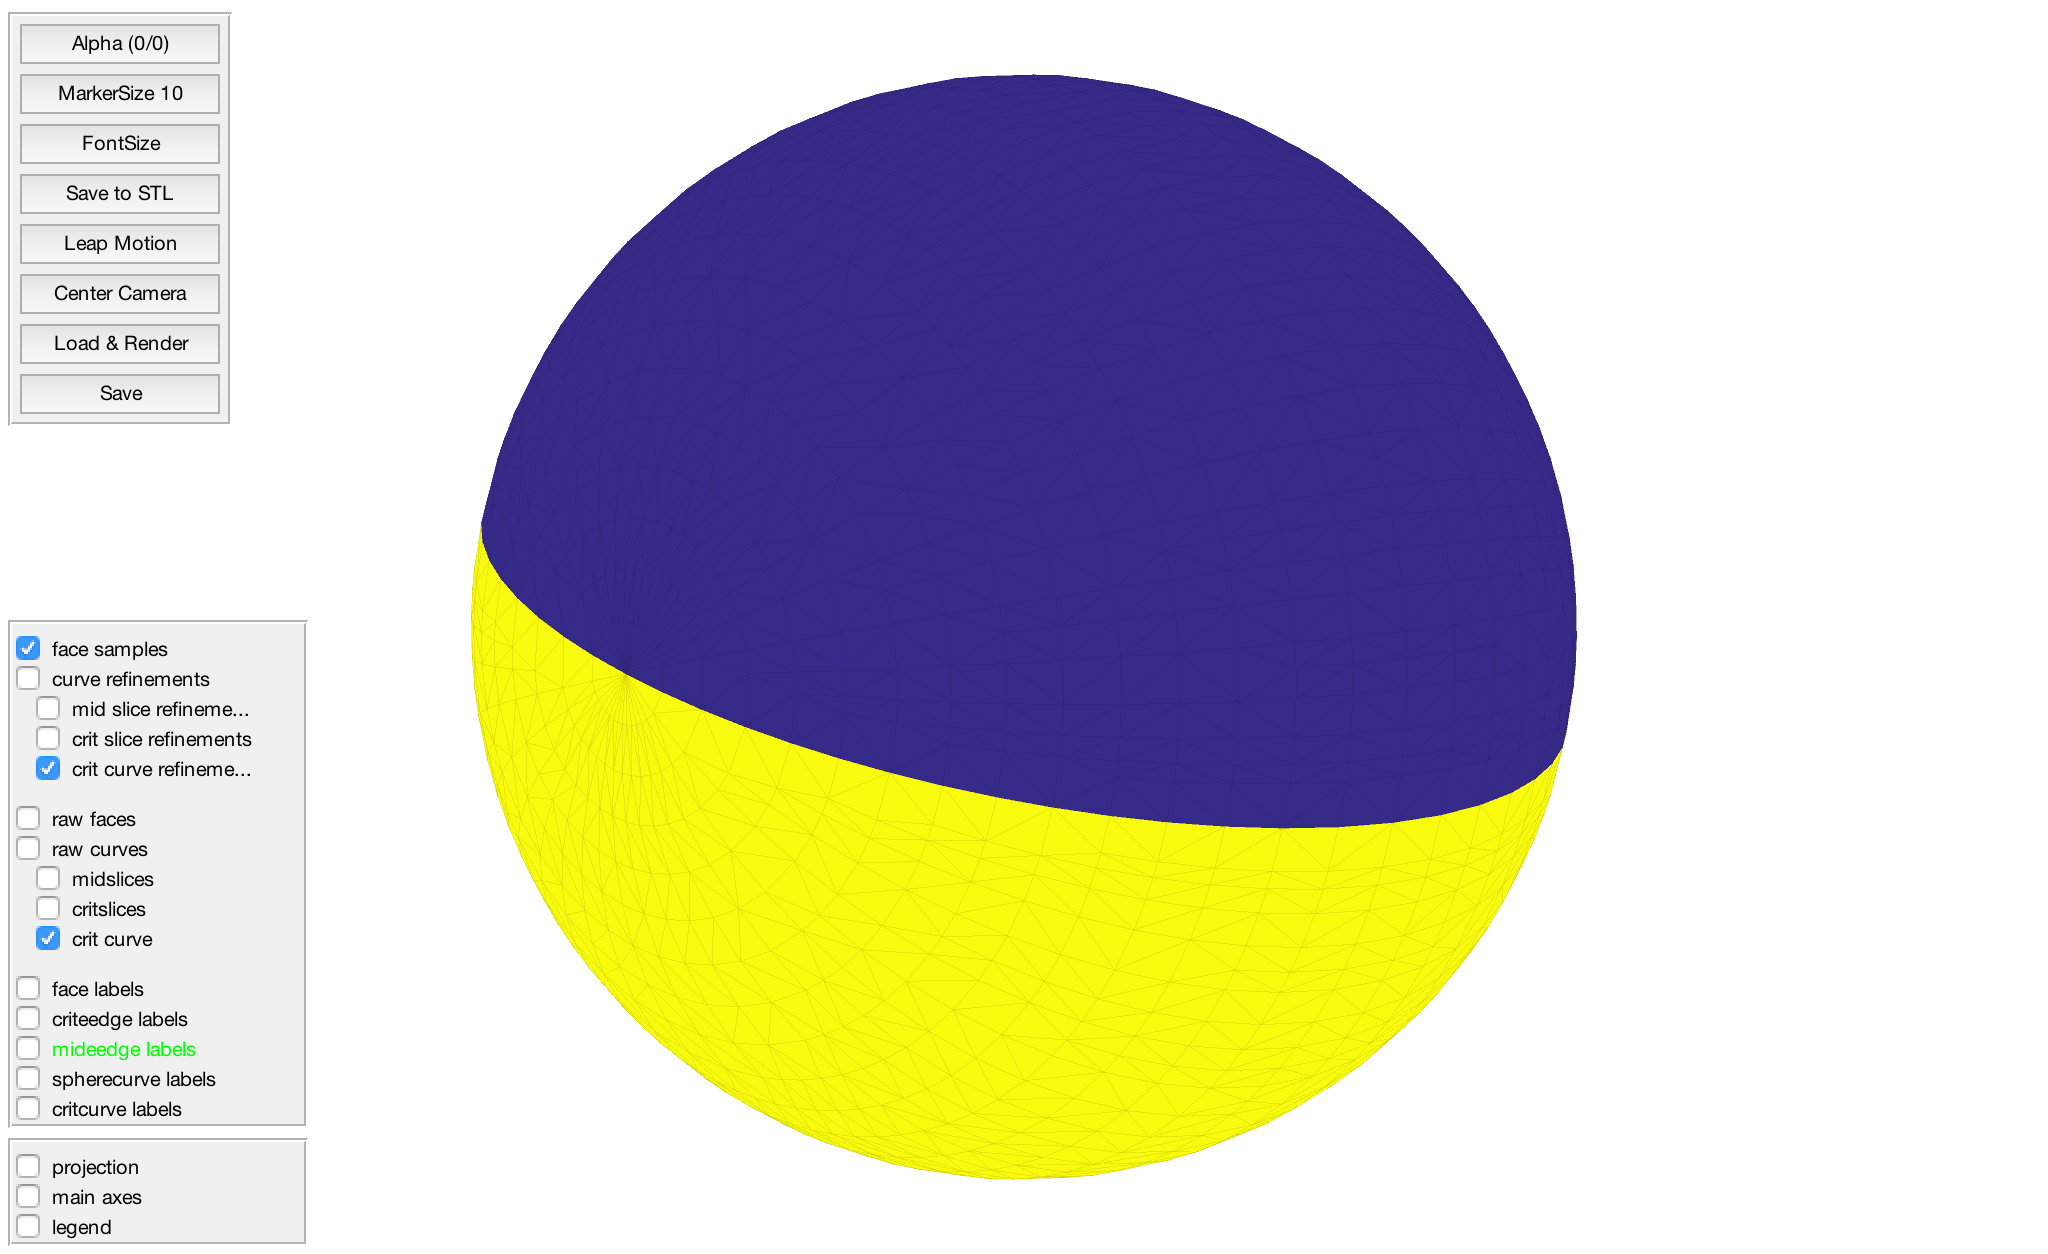
\includegraphics [width=0.4\textwidth]{surfacesampler2} \\ \\ \\   
\end{longtabu}






\subsubsection{Available surface sampling algorithms}


There are currently about two surface sampling algorithms, one of which is generally far superior to the other.  The inferior method is left for posterity, because it produces interesting patterns on some surfaces.  

\begin{enumerate}
\item {\tt -m a} – Adaptive – Default choice.  Will be adaptive on distance moved, once it's implemented.  Sorry, we're not there yet on this one.
\item {\tt -m d} – Adaptive – Also default choice, because adaptive-movement collapses to the adaptive-distance method, until movement is implemented.  The sampling of critical-like curves are non-uniform, having somewhat-uniformly spaced samplings in terms of projection value across the entire curve.  Slices and ribs are distance-adaptively sampled.
\item {\tt -m f} – Fixed – every edge of every critical-like curve gets the same number of points, and slices and ribs are sampled distance-adaptively.
\end{enumerate}

In short, the difference between distance-adaptive and fixed sampling is twofold:
\begin{itemize}

  \item Fixed sampling has the same number of ribs on each face, regardless of size

  \item Adaptive sampling spaces the ribs by cycle number, better approximating regions of the surface coming together at a singularity or critical point.

\end{itemize}


In all surface sampling algorithms, new points in the surface are computed by exploiting the homotopy \eqref{eqn:midtrack} from Section~\ref{sec:connect_surface}.  We will first discuss the weaker of the two methods, because it is briefer and easier to explain.

\paragraph{Surface sampling algorithm: Fixed}

In the fixed-number surface sampling algorithm, 


\paragraph{Surface sampling algorithm: Adaptive by distance}

 This means that wider edges will have more samples.  However, all edges in a single projection interval will have the same number of samples.  They are also scaled by the cycle number (this is a lie, the cycle number is fixed at 2 due to technical reasons for now).


